\usepackage{graphicx}
\usepackage{wasysym}
\newpage
\thispagestyle{fancy}
\vspace{\fill}

\subsection{\small Velocidade da máquina}
\begin{figure}
    \centering
    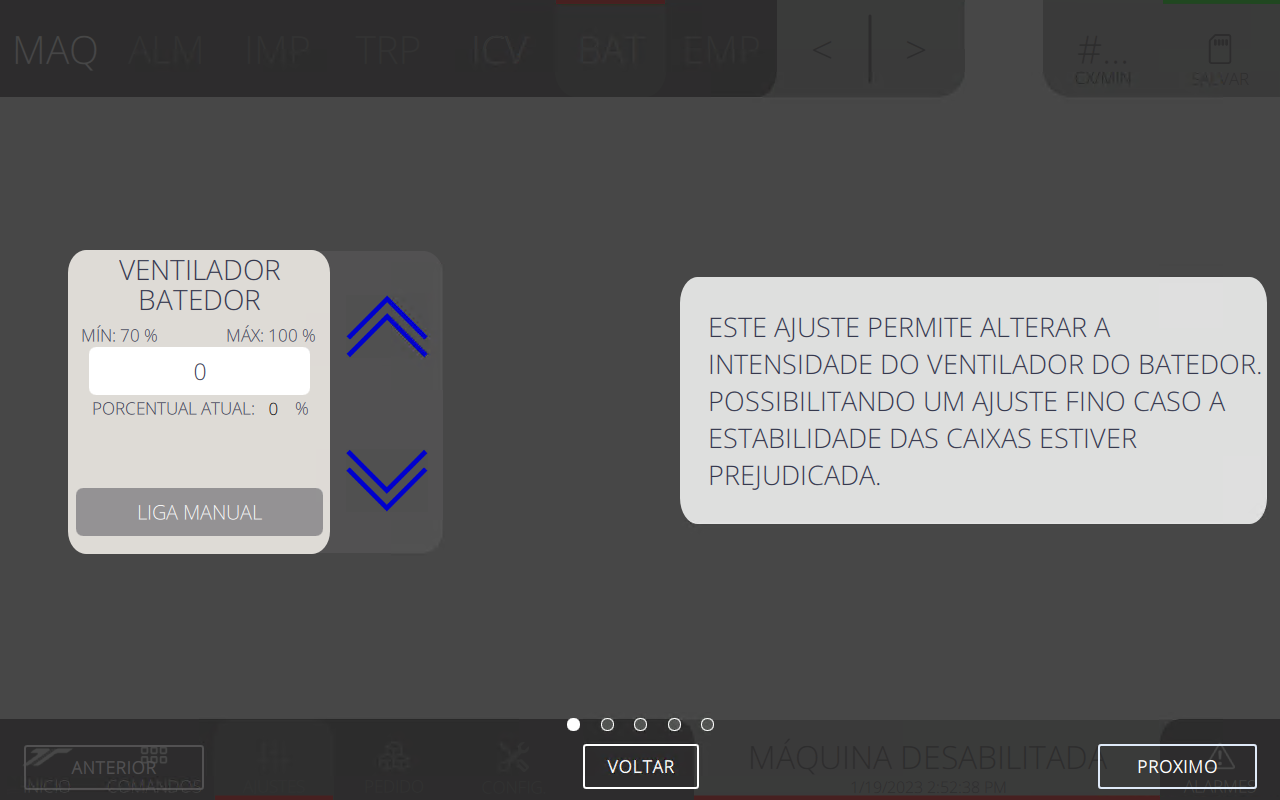
\includegraphics[width=480,height=300]{imagesICV/08-stacker/commands/e-1}
    \caption{Velocidade da máquina}
\end{figure}
\newpage

\thispagestyle{fancy}
\vspace{\fill}
\subsection{\small Habilita ventilador 2}
\begin{figure}
    \centering
    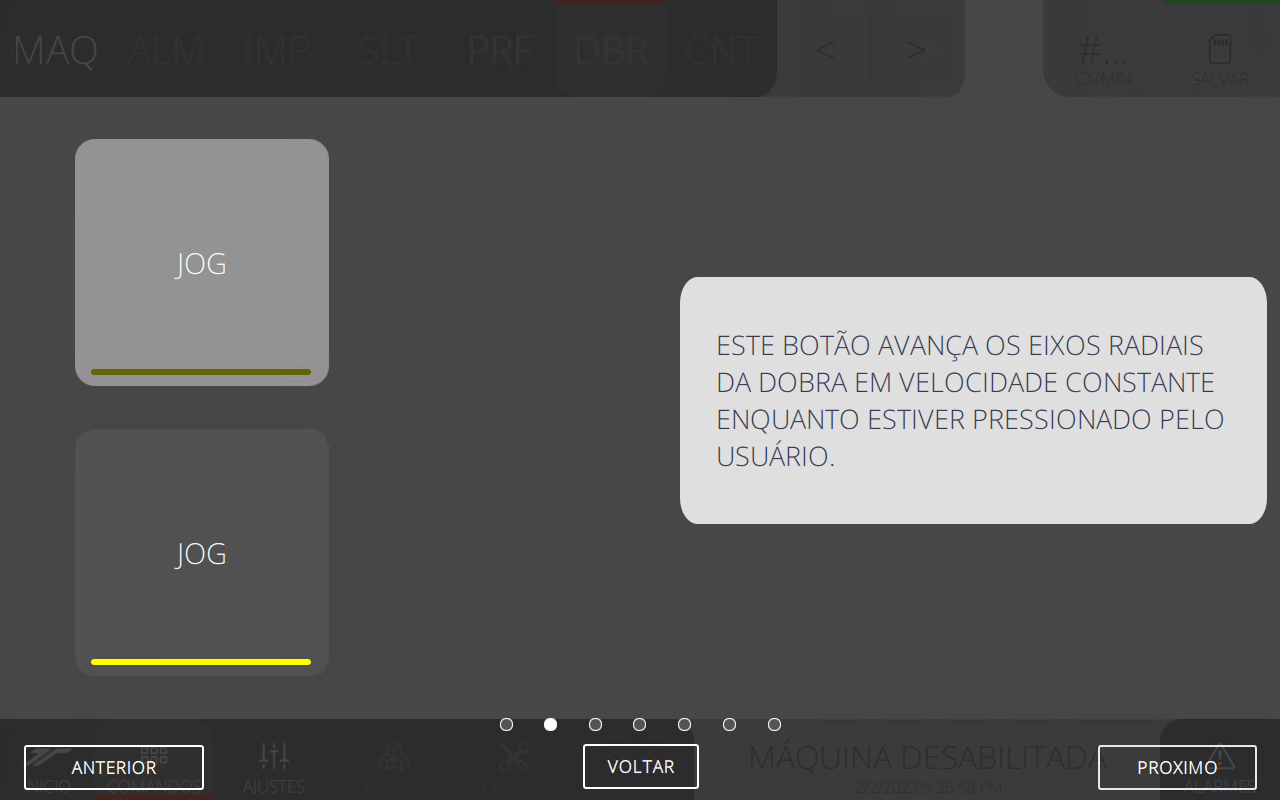
\includegraphics[width=576,height=360]{imagesICV/08-stacker/commands/e-2}
    \caption{}
\end{figure}
\newpage

\thispagestyle{fancy}
\vspace{\fill}
\subsection{\small Desabilita ventilador 1}
\begin{figure}
    \centering
    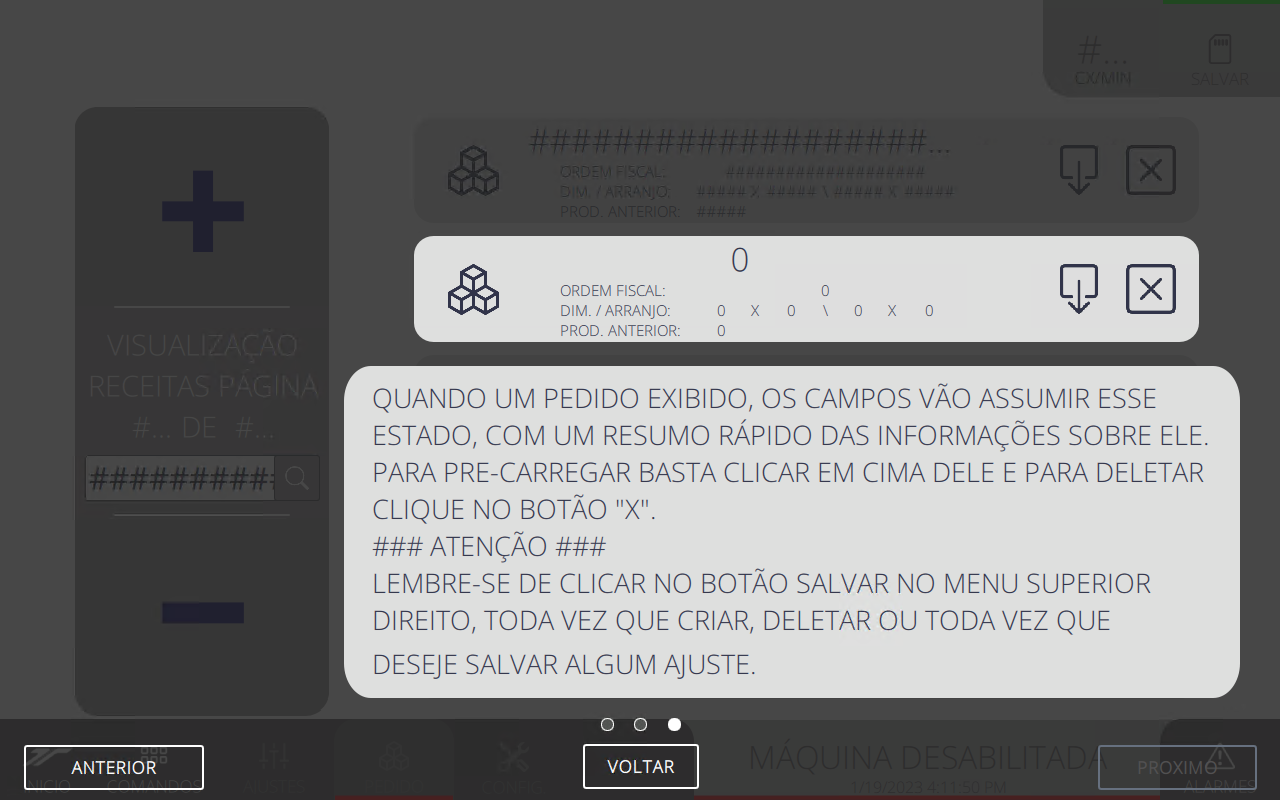
\includegraphics[width=576,height=360]{imagesICV/08-stacker/commands/e-3}
    \caption{Desabilita ventilador 1}
    \label{}
\end{figure}
\newpage

\thispagestyle{fancy}
\vspace{\fill}
\subsection{\small Executa ponto zero da unidade}
\begin{figure}
    \centering
    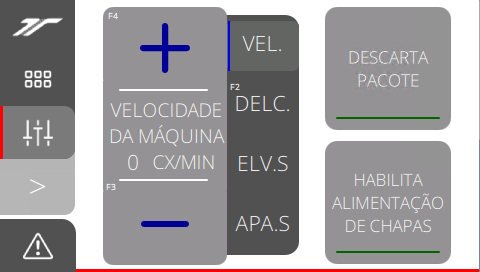
\includegraphics[width=576,height=360]{imagesICV/08-stacker/commands/e-4}
    \caption{Executa ponto zero da unidade}
    \label{}
\end{figure}
\newpage

\thispagestyle{fancy}
\vspace{\fill}
\subsection{\small Habilita roletes}
\begin{figure}
    \centering
    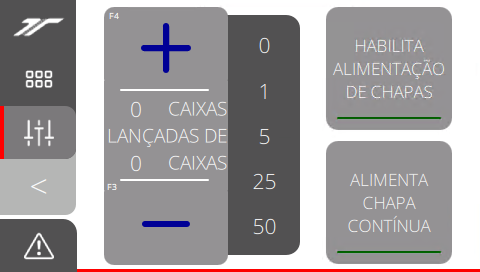
\includegraphics[width=576,height=360]{imagesICV/08-stacker/commands/e-5}
    \caption{Habilita roletes}
    \label{fig:}
\end{figure}
\newpage

\thispagestyle{fancy}
\vspace{\fill}
\subsection{\small Habilita movimento dos eixos}
\begin{figure}
    \centering
    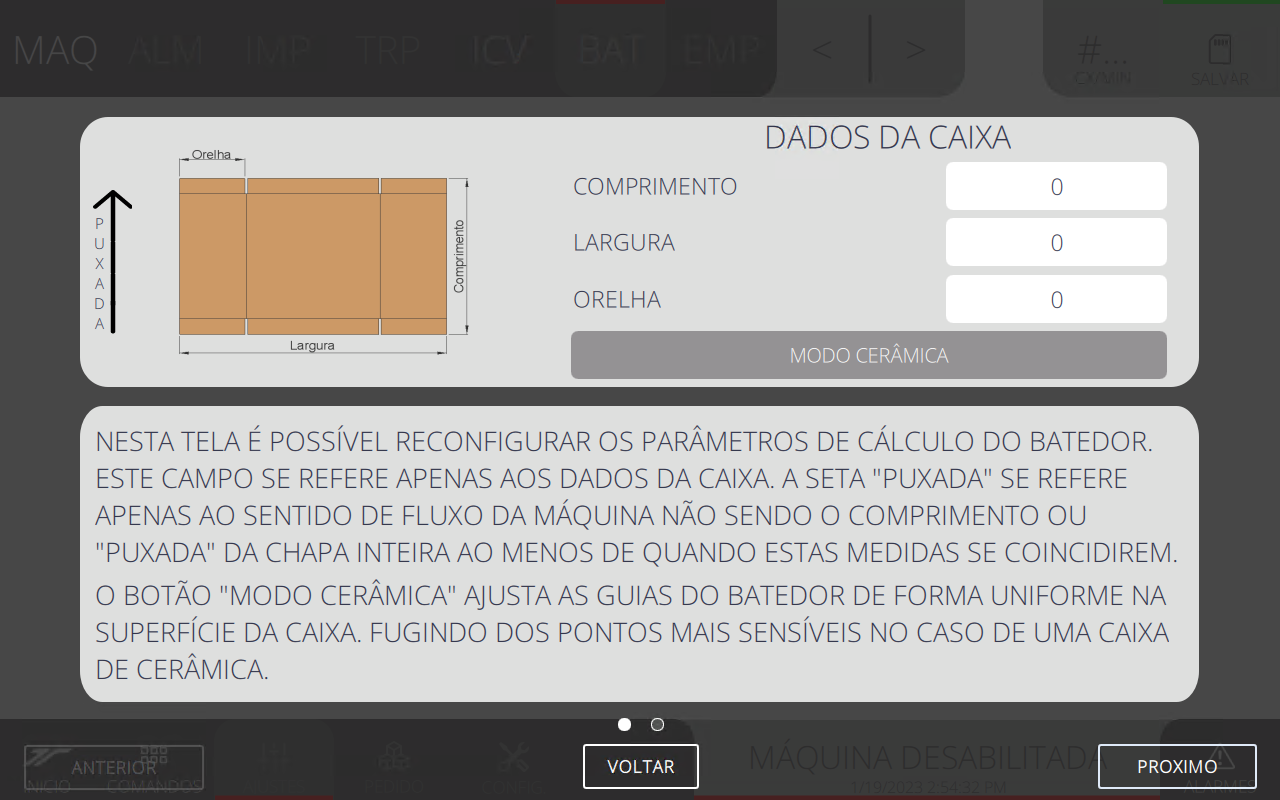
\includegraphics[width=576,height=360]{imagesICV/08-stacker/commands/e-6}
    \caption{Habilita movimento dos eixos}
\end{figure}
\newpage

\thispagestyle{fancy}
\vspace{\fill}
\subsection{\small Executa ponto zero altura batente das caixas}
\begin{figure}
    \centering
    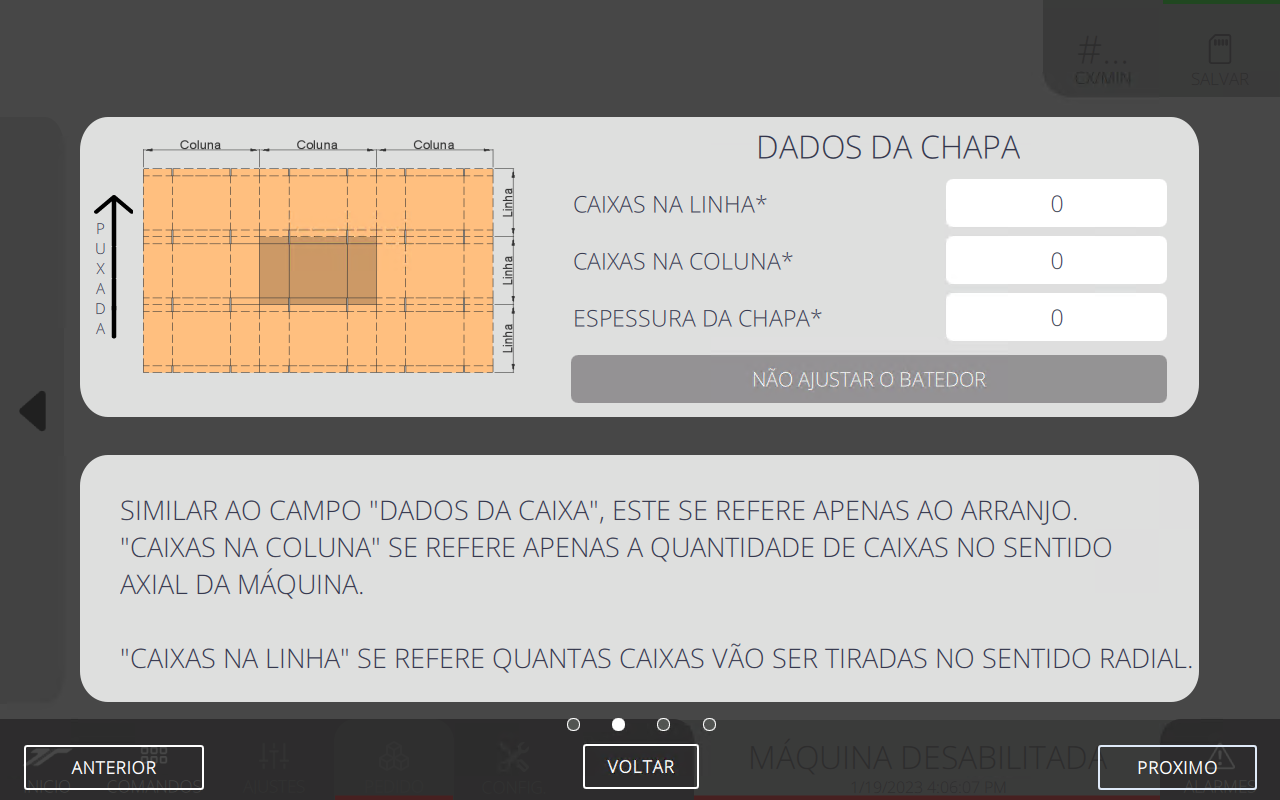
\includegraphics[width=576,height=360]{imagesICV/08-stacker/commands/e-7}
    \caption{Executa ponto zero altura batente das caixas}
\end{figure}
\newpage

\thispagestyle{fancy}
\vspace{\fill}
\subsection{\small Habilita função Jog}
\begin{figure}
    \centering
    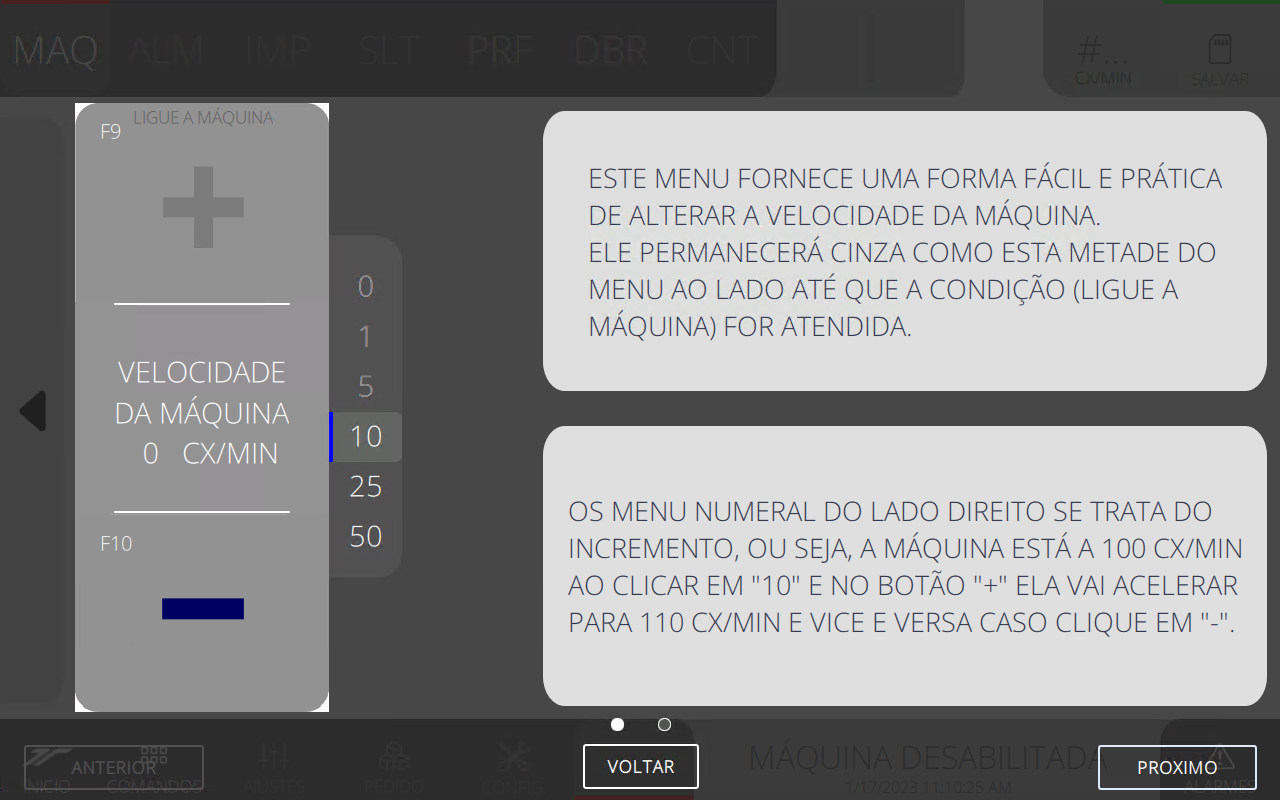
\includegraphics[width=576,height=360]{imagesICV/08-stacker/commands/e-8}
    \caption{Habilita função Jog}
\end{figure}
\newpage

\thispagestyle{fancy}
\vspace{\fill}
\subsection{\small Movimento incial dos eixos}
\begin{figure}
    \centering
    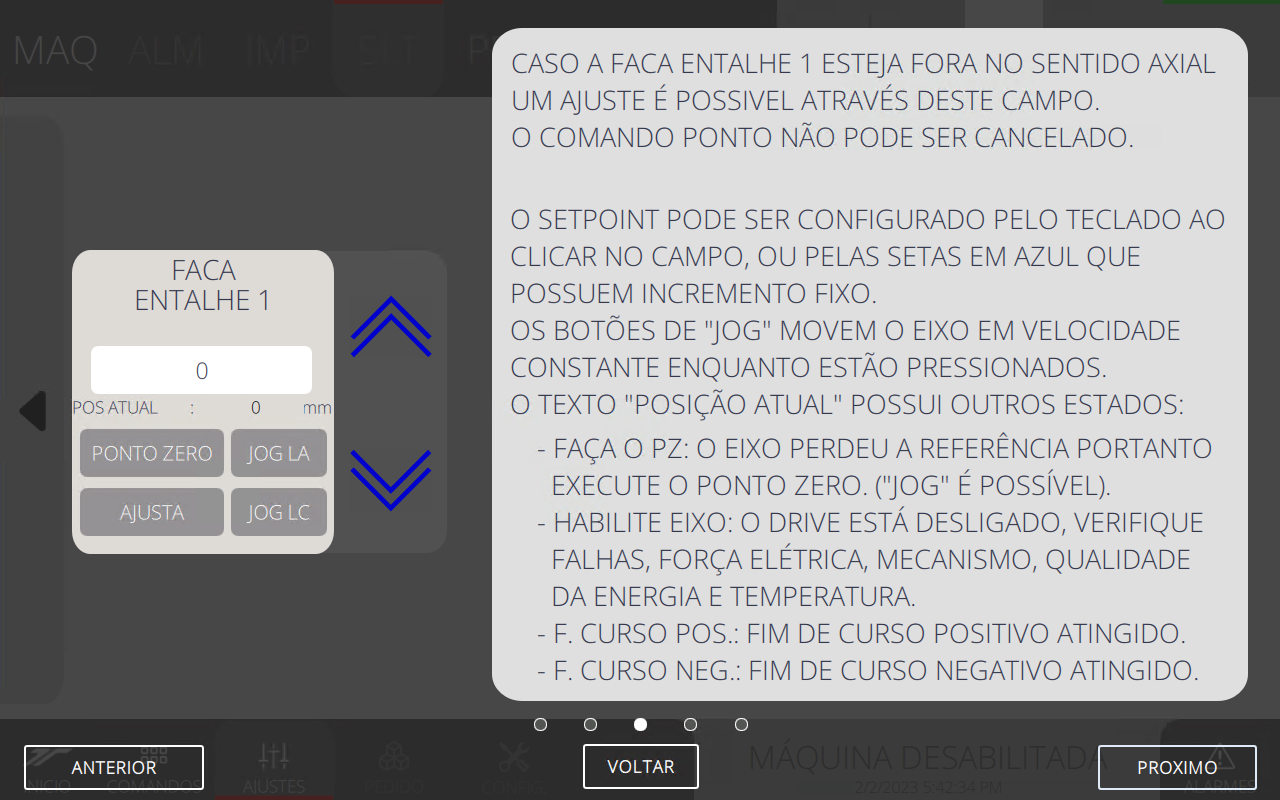
\includegraphics[width=576,height=360]{imagesICV/08-stacker/commands/e-9}
    \caption{Movimento incial dos eixos}
\end{figure}
\newpage

\thispagestyle{fancy}
\vspace{\fill}
\subsection{\small Descarta pilha}
\begin{figure}
    \centering
    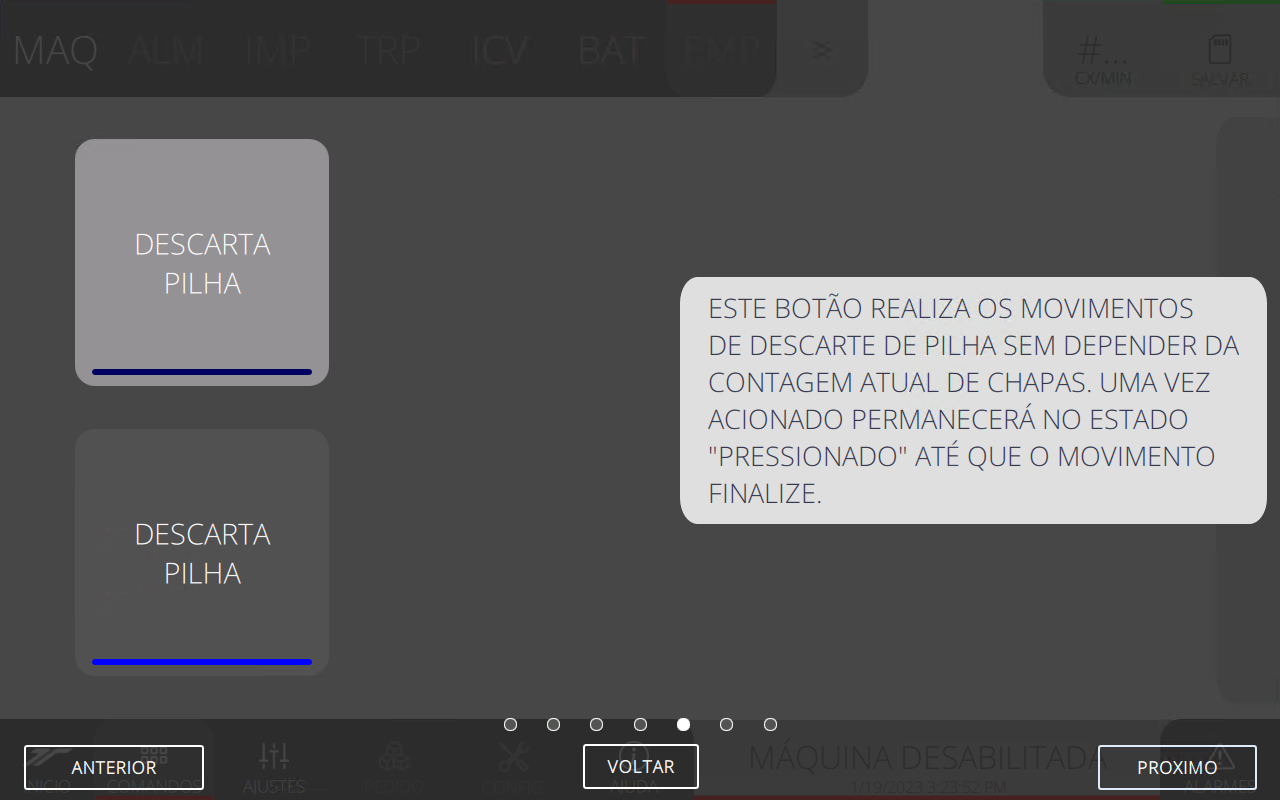
\includegraphics[width=576,height=360]{imagesICV/08-stacker/commands/e-10}
    \caption{Descarta pilha}
\end{figure}
\newpage

\thispagestyle{fancy}
\vspace{\fill}
\subsection{\small Desabilita modo embuchamento}
\begin{figure}
    \centering
    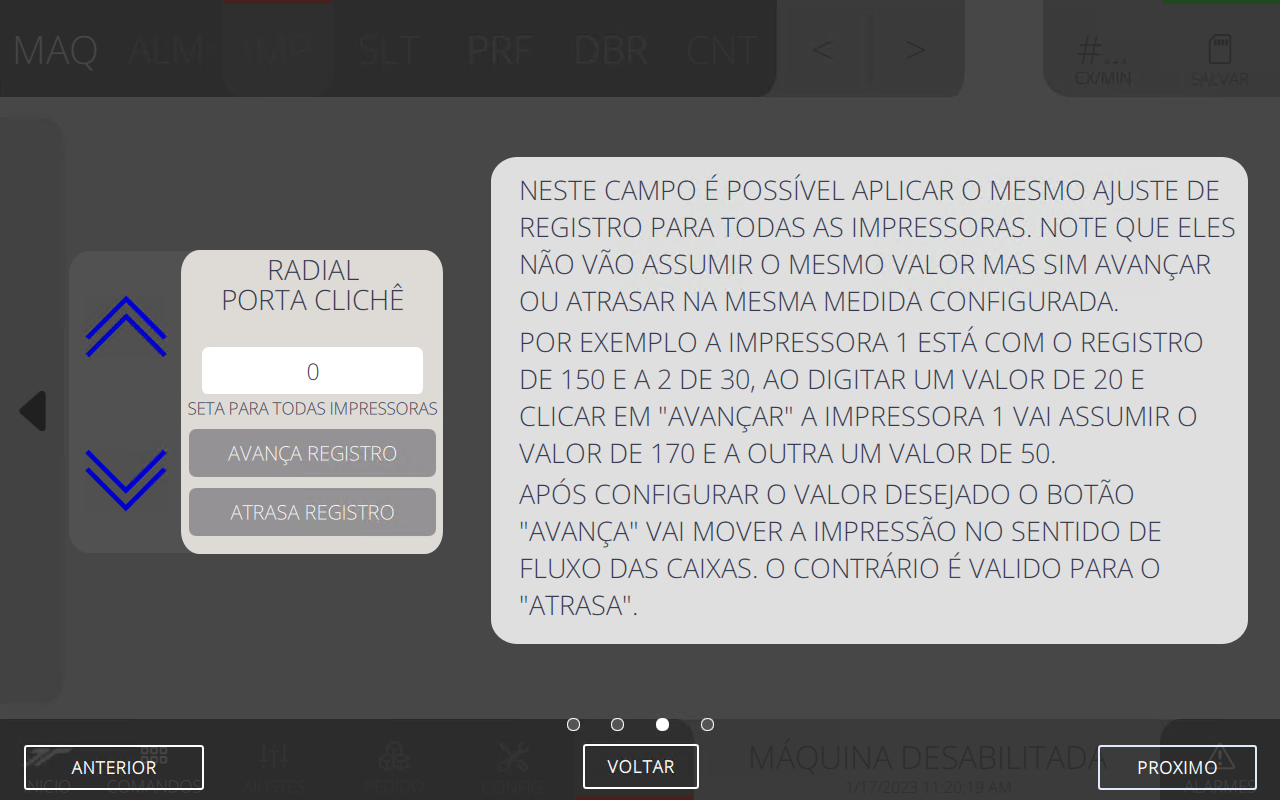
\includegraphics[width=576,height=360]{imagesICV/08-stacker/commands/e-11}
    \caption{Desabilita modo embuchamento}
\end{figure}
\newpage

\thispagestyle{fancy}
\vspace{\fill}
\subsection{\small Separa pilha}
\begin{figure}
    \centering
    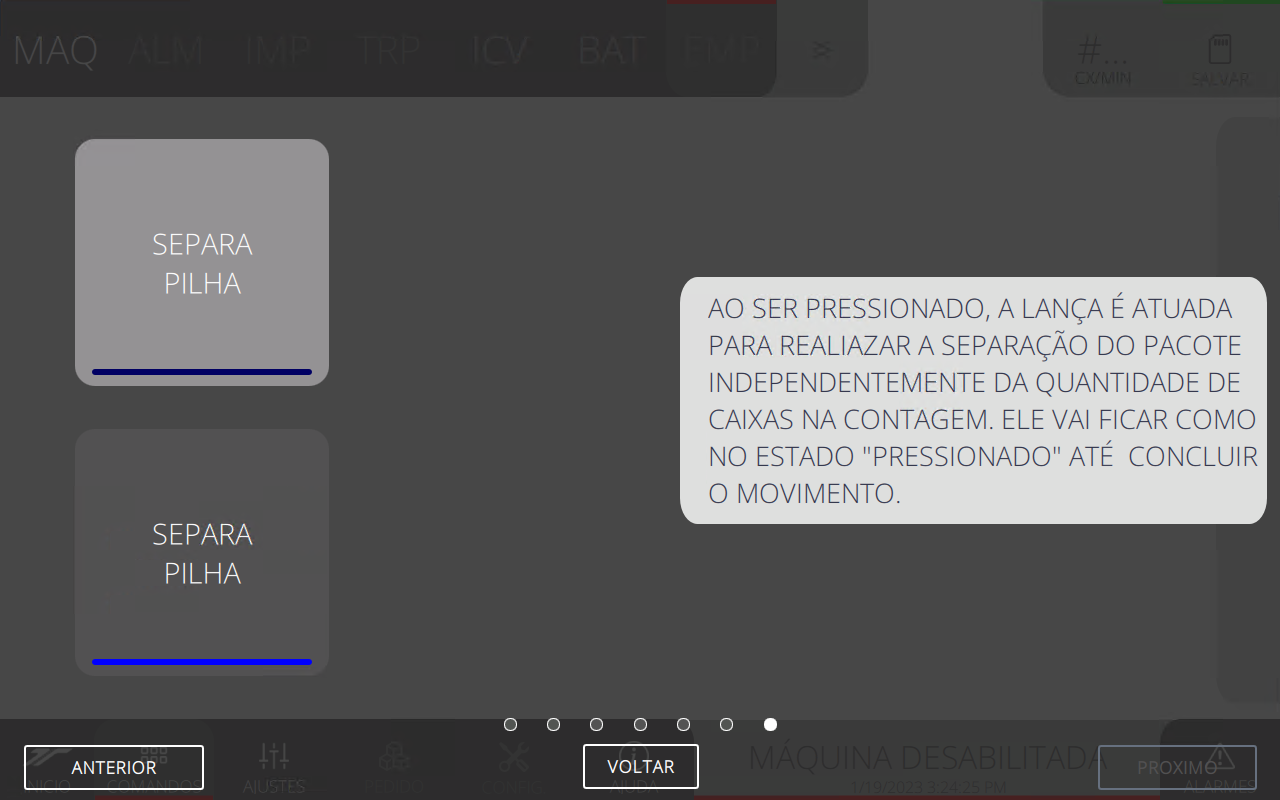
\includegraphics[width=576,height=360]{imagesICV/08-stacker/commands/e-12}
    \caption{Separa pilha}
\end{figure}

